% ICASSP 2027 conference manuscript.
% Uses the official ICASSP 2027 spconf.sty and IEEEbib.bst.
% Overleaf compiler: pdfLaTeX.
%
% Required project files:
%   spconf.sty
%   IEEEbib.bst
%   refs.bib
%   figures/heatmap_lpips_output_mean_cr040_050_cond_vs_uncond_j10.png

\documentclass{article}

\usepackage{spconf}
\usepackage{amsmath,amssymb}
\usepackage{graphicx}
\usepackage{booktabs}
\usepackage{cite}
\usepackage{url}
\usepackage[hidelinks]{hyperref}

\title{Resampling Is Not Always Better: Conditioning Flips the Effect of RePaint Jumps}

\name{Hussein Hamouda}

\address{
Purdue University, West Lafayette, IN, USA\\
hanafy@purdue.edu
}

\begin{document}

\ninept
\maketitle

\begin{abstract}
RePaint uses repeated forward--backward jumps to harmonize known and generated pixels during diffusion inpainting. We show that this resampling is not universally beneficial. Under paired, seed-matched evaluation on CelebA, increasing the resampling count degrades a mask-conditioned DDPM by about $2.7$ dB PSNR on large center holes, while improving an unconditional DDPM by $1.6$--$2.2$ dB. A matched-coverage brush-mask control shows no significant effect, indicating that the conditioned degradation depends on contiguous-hole geometry rather than masked area alone. An external qualitative check using RePaint's released unconditional checkpoint is consistent with the unconditional trend. Since inference cost scales nearly linearly with resampling, the best setting for the conditioned model is also the cheapest. These results show that RePaint resampling should be selected according to the model's conditioning regime rather than transferred as a universal inference default.
\end{abstract}

\begin{keywords}
diffusion models, image inpainting, RePaint, resampling, conditional generation
\end{keywords}


\section{Introduction}
\label{sec:intro}

Diffusion models are widely used for image restoration and inpainting.
In an unconditional denoising diffusion probabilistic model (DDPM)~\cite{ho2020ddpm},
the network does not observe the inpainting mask during training, so known pixels
must be enforced during inference.
RePaint~\cite{lugmayr2022repaint} addresses this by reinserting noise-matched
known pixels after reverse steps and optionally applying repeated forward--backward
jumps. The number of resampling passes, denoted $r$, gives the unconditional
prior additional opportunities to reconcile the generated hole with its context.

A different regime trains the diffusion network to observe the masked image and
mask directly, as in Palette-style conditional diffusion~\cite{saharia2022palette}.
The same RePaint $(j,r)$ inference recipe can nevertheless be applied to such a
model. This raises a simple question: does additional RePaint resampling remain
beneficial when the denoiser has already been trained to use the known-pixel
constraint?

We find that the answer depends strongly on the training regime.
Under paired, seed-matched CelebA~\cite{liu2015celeba} experiments, increasing
$r$ has opposite effects for conditioned and unconditional DDPMs.
For large contiguous center holes, increasing $r$ substantially degrades the
mask-conditioned model but improves the unconditional model.
A matched-coverage brush-mask control shows no significant degradation,
indicating that the effect is not explained by missing-pixel count alone.
A qualitative check with RePaint's released unconditional CelebA-HQ checkpoint
is also consistent with the unconditional trend.

Our contribution is therefore an empirical boundary condition on RePaint
resampling: the same inference-time mechanism that improves an unconditional
prior can become redundant or harmful when an explicit conditioning channel
already carries the measurement constraint. This observation is distinct from
adaptive resampling methods such as StrDiffusion~\cite{liu2024strdiffusion},
which modify resampling according to learned structural information.


\section{Method and Evaluation}
\label{sec:method}

\subsection{Models and Training}

We compare two $\varepsilon$-prediction DDPMs with the same U-Net capacity:
base width $64$, channel multipliers $(1,2,4)$, two residual blocks per level,
self-attention at $16{\times}16$, and dropout $0.1$.
Both use a linear $T{=}1000$ diffusion schedule with
$\beta_t\in[10^{-4},0.02]$ and are trained on CelebA images resized to
$64{\times}64$ using Adam with learning rate $2{\times}10^{-4}$ and batch size
$32$. Quantitative results use the epoch-$30$ checkpoints.

The \emph{conditioned} model predicts noise from
$(x_t,\tilde{x}_0,m)$, where
$\tilde{x}_0=m\odot x_0$ contains the known pixels and
$m$ denotes the known-pixel mask.
During training it receives center, rectangle, brush, and holes masks.
The \emph{unconditional} model receives only $x_t$ and is trained on clean
images, so the mask enters only through the inference procedure.
Additional training and protocol details follow our earlier technical
report~\cite{hamouda2026protocol}.

\subsection{RePaint Resampling}

After a reverse step produces a candidate unknown-region estimate
$\hat{x}_{t-1}^{\mathrm{unk}}$, RePaint forms the noise-matched stitch

\begin{equation}
x_{t-1}
=
m\odot q(x_0,t{-}1)
+
(1-m)\odot\hat{x}_{t-1}^{\mathrm{unk}},
\label{eq:stitch}
\end{equation}

where $q(x_0,t{-}1)$ forward-diffuses the known pixels to the appropriate noise
level~\cite{lugmayr2022repaint}.
For $r>1$, RePaint additionally applies forward jumps and subsequently
denoises and stitches again:

\begin{equation}
x_t=
\sqrt{1-\beta_t}\,x_{t-1}
+
\sqrt{\beta_t}\,\varepsilon,
\qquad
\varepsilon\sim\mathcal{N}(0,I).
\label{eq:jump}
\end{equation}

Setting $r{=}1$ therefore retains the known-pixel stitch but disables additional
resampling jumps.

\subsection{Paired Evaluation Protocol}

Headline experiments use the full reverse schedule $T{=}1000$, jump length
$j{=}10$, and center masks with side ratios
$\mathrm{cr}\in\{0.40,0.50\}$.
We evaluate $r\in\{1,5,10\}$.
Each setting uses the same $n{=}32$ CelebA validation identities.
Before processing sample $i$, we reseed the random number generator with
$42+i$; paired settings therefore start from the same $x_T$ and use
corresponding stochastic noise streams rather than allowing larger $r$ to
desynchronize subsequent samples.

We record image-wide PSNR and LPIPS~\cite{zhang2018lpips}.
For the conditioned model, headline differences compare $r{=}10$ with $r{=}1$;
for the unconditional model they compare $r{=}5$ with $r{=}1$, corresponding
to the best operating points observed in the resampling sweep.
Positive $\Delta$PSNR and negative $\Delta$LPIPS indicate improvement.


\section{Results}
\label{sec:results}

\subsection{Conditioning Flips the Effect of Resampling}

Table~\ref{tab:main} shows the paired effect of increasing $r$.
For the mask-conditioned model, $r{=}1\rightarrow10$ reduces PSNR by
$2.73$ dB at both center-mask sizes.
The effects are large
($d=-1.08$ and $-1.16$) and highly significant
($p<10^{-6}$), while LPIPS also worsens.

The unconditional model exhibits the opposite behavior.
Increasing $r$ from $1$ to $5$ improves PSNR by $2.22$ dB at
$\mathrm{cr}{=}0.40$ and $1.58$ dB at $\mathrm{cr}{=}0.50$,
with $p<0.01$ in both cases.
LPIPS decreases accordingly.

\begin{table*}[t]
\centering
\caption{Paired effect of increasing RePaint resampling
($n{=}32$, $j{=}10$, $T{=}1000$).
Conditioned:
$\Delta=\mathrm{metric}(r{=}10)-\mathrm{metric}(r{=}1)$.
Unconditional:
$\Delta=\mathrm{metric}(r{=}5)-\mathrm{metric}(r{=}1)$.
Positive $\Delta$PSNR and negative $\Delta$LPIPS indicate improvement.}
\label{tab:main}
\setlength{\tabcolsep}{4.5pt}
\begin{tabular}{llccccc}
\toprule
Model & Mask &
$\Delta$PSNR (dB) &
95\% CI &
$\Delta$LPIPS &
$p$ (PSNR) &
Cohen's $d$ \\
\midrule
Conditioned   & $0.40$ & $-2.73$ & $[-3.64,-1.81]$ & $+0.0234$ & $9.5{\times}10^{-7}$ & $-1.08$ \\
Conditioned   & $0.50$ & $-2.73$ & $[-3.58,-1.88]$ & $+0.0340$ & $2.6{\times}10^{-7}$ & $-1.16$ \\
Unconditional & $0.40$ & $+2.22$ & $[0.67,3.78]$   & $-0.0106$ & $6.6{\times}10^{-3}$ & $+0.51$ \\
Unconditional & $0.50$ & $+1.58$ & $[0.48,2.69]$   & $-0.0161$ & $6.5{\times}10^{-3}$ & $+0.52$ \\
\bottomrule
\end{tabular}
\end{table*}

Figure~\ref{fig:heatmap} shows the full $r\in\{1,5,10\}$ LPIPS sweep.
For the conditioned model, $r{=}1$ is best and quality worsens monotonically
as $r$ increases.
For the unconditional model, quality improves from $r{=}1$ to $r{=}5$;
$r{=}10$ remains better than $r{=}1$ but is slightly worse than $r{=}5$.

\begin{figure*}[t]
\centering
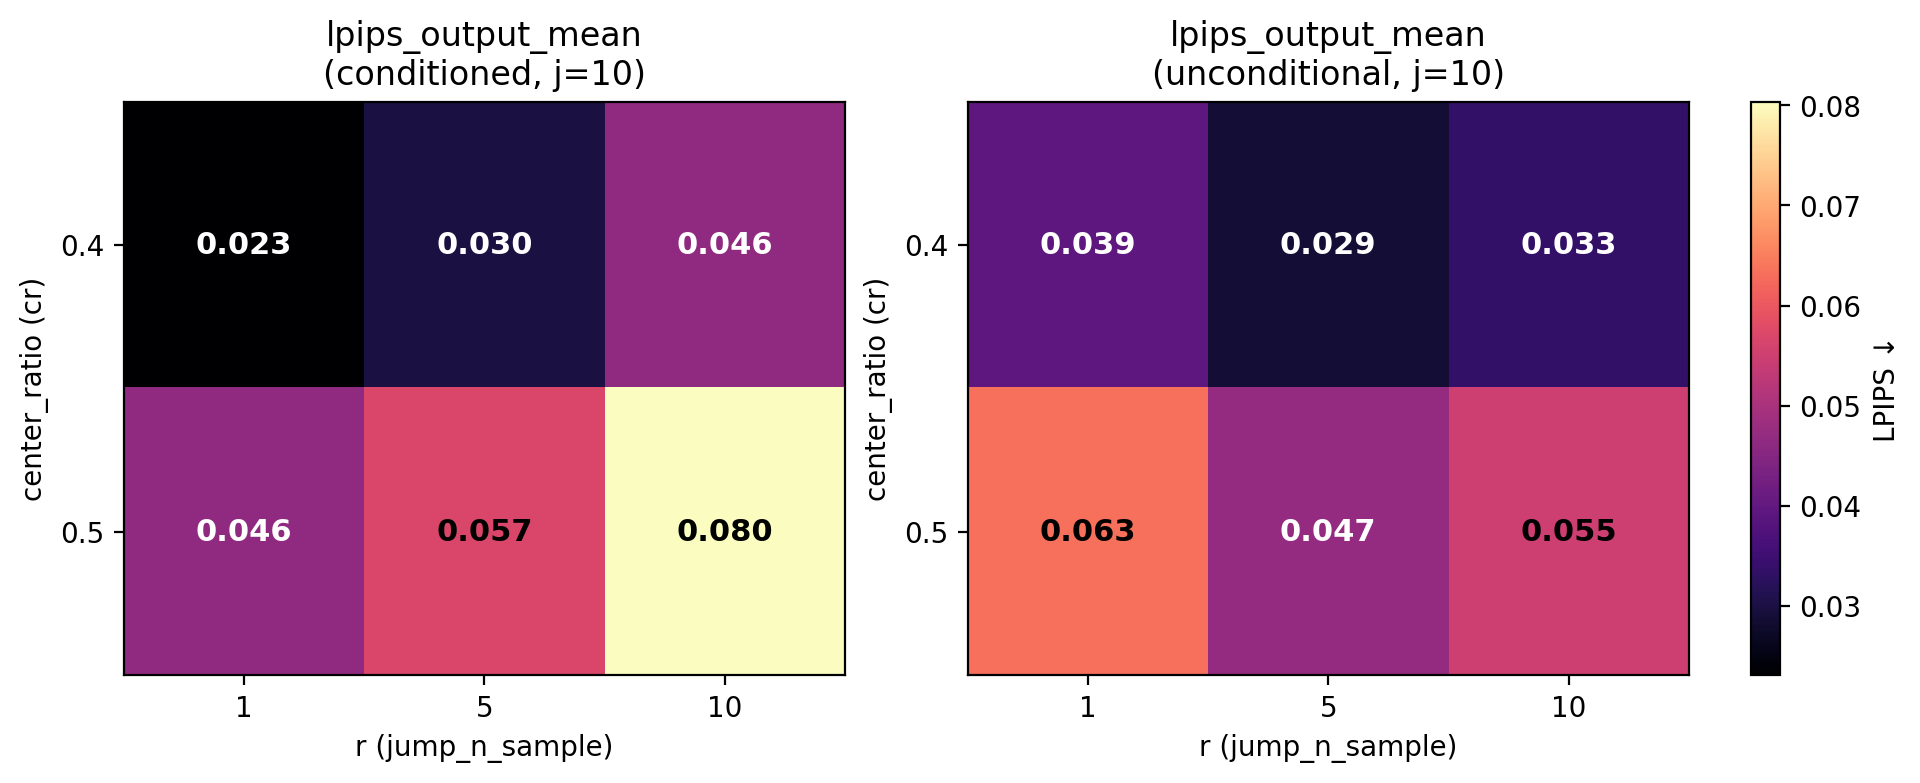
\includegraphics[
    width=0.86\textwidth,
    height=1.55in,
    keepaspectratio
]{figures/heatmap_lpips_output_mean_cr040_050_cond_vs_uncond_j10.png}
\caption{Mean LPIPS (lower is better) versus resampling count $r$
for center-mask inpainting at $j{=}10$.
Left: conditioned DDPM.
Right: unconditional DDPM.
The trends have opposite directions.}
\label{fig:heatmap}
\end{figure*}


\subsection{Geometry Control and External Check}

To test whether the conditioned degradation is caused simply by the number of
missing pixels, we evaluate brush masks with coverage matched to a
$\mathrm{cr}{=}0.40$ center hole.
Using the same paired protocol with $r{=}10$ versus $r{=}1$,
PSNR changes by only $+0.30$ dB
(95\% CI $[-0.61,+1.20]$, $p{=}0.51$, $d{=}0.12$);
LPIPS changes by $+0.0006$ ($p{=}0.25$, $d{=}0.21$).
Thus, increasing $r$ has no statistically significant effect for sparse,
non-contiguous missing regions at matched coverage.
The conditioned degradation is therefore associated with large contiguous
holes rather than masked area alone.

We additionally evaluate RePaint's publicly released unconditional CelebA-HQ
checkpoint at $256{\times}256$ using a respaced $T{=}100$ schedule,
$j{=}10$, and $r\in\{1,5,10\}$ on eight samples.
This check is qualitative rather than part of Table~\ref{tab:main};
higher $r$ improves seam consistency and does not show the degradation observed
for our conditioned model.
This provides an external consistency check that the unconditional benefit is
not specific to our $64{\times}64$ architecture.

\subsection{Inference Cost}

The computational cost grows almost linearly with the resampling count.
At $T{=}1000$ and $j{=}10$, $r{=}1$, $5$, and $10$ require
$1000$, $4960$, and $9910$ network function evaluations, respectively.
Measured wall-clock time increases from $14.1$ s/image at $r{=}1$ to
$70.8$ s/image at $r{=}5$ and $149.7$ s/image at $r{=}10$.
Thus, for the conditioned model, increasing $r$ can simultaneously reduce
quality and increase inference cost by approximately an order of magnitude.


\section{Discussion}
\label{sec:discussion}

The results suggest a simple explanation based on how the known-pixel
constraint enters each model.
In unconditional RePaint,
$\varepsilon_\theta=\varepsilon_\theta(x_t,t)$: the denoiser never sees the
mask or known image directly.
The stitch in~\eqref{eq:stitch} enforces measurement consistency only after a
reverse update, while the jump in~\eqref{eq:jump} reopens the generation process
so that denoising and constraint enforcement can be repeated.
Resampling can therefore be viewed as a projection-style correction mechanism
that supplies information absent from the unconditional network.

The conditioned predictor instead evaluates
$\varepsilon_\theta(x_t,t,\tilde{x}_0,m)$ at every reverse step.
The known image and mask are already static conditioning channels that steer
the reverse process.
We hypothesize that repeatedly adding RePaint jumps on top of this learned
conditioning is largely redundant.
For a large contiguous hole, repeated re-noising and re-denoising can overwrite
a coherent completion already established by the conditioned predictor,
producing the observed over-harmonized degradation.
The brush-mask null is consistent with this interpretation because sparse
missing regions retain dense local context and provide less coherent interior
area for repeated resampling to rewrite.

This mechanism is an interpretation of paired ablations rather than a formal
proof.
The experiments use one U-Net capacity, one epoch-$30$ checkpoint per regime,
$64{\times}64$ CelebA, and $n{=}32$ paired images.
The conditioned model is evaluated here at the full $T{=}1000$ schedule;
whether the effect persists under coarser respaced schedules remains open.
Larger datasets, latent-diffusion inpainting systems, and additional mask
families should therefore be tested before treating $r{=}1$ as a universal
rule for all conditioned diffusion models.


\section{Conclusion}
\label{sec:conclusion}

RePaint resampling has opposite effects under two diffusion-inpainting training
regimes: it improves an unconditional DDPM but degrades a mask-conditioned DDPM
on large contiguous holes.
A matched-coverage brush control shows that the conditioned harm is not explained
by masked area alone, while an external RePaint checkpoint is consistent with
the unconditional trend.
Because resampling also multiplies inference cost, $(j,r)$ should be selected
together with the model's conditioning regime rather than transferred as a
universal inference default.


% ----------------------------------------------------------------------
% ICASSP requires funding/conflict and ethical-compliance disclosures.
% These may appear on page 5 together with the references.
%
% IMPORTANT:
% Add the accurate funding statement before submission.
% Do not claim "no funding" unless that is actually true.
% ----------------------------------------------------------------------

\section*{Acknowledgment}

% TODO: Insert the accurate funding disclosure here.
% Example ONLY if true:
% No funding was received for conducting this study.

The author declares no relevant financial or nonfinancial conflicts of interest.


\section*{Compliance with Ethical Standards}

This study uses the publicly available CelebA dataset and involved no new data
collection or interaction with human participants.

% TODO BEFORE SUBMISSION:
% Confirm the exact ethics-review / waiver wording applicable to your
% institution and dataset use, and add it above if required.


\bibliographystyle{IEEEbib}
\bibliography{refs}

\end{document}